
\title{SOME ARITHMETICAL DISCRETE GROUPS IN LOBA$\hat{\text{C}}$EVSKI$\hat{\text{I}}$ SPACES}
\markright{SOME ARITHMETICAL DISCRETE GROUPS IN LOBA$\hat{\text{C}}$EVSKI$\hat{\text{I}}$ SPACES}

\author{By~ \`E. B. VINBERG}
\markboth{\'E. B. VINBERG}{SOME ARITHMETICAL DISCRETE GROUPS IN LOBA$\hat{\text{C}}$EVSKI$\hat{\text{I}}$ SPACES}

\date{}
\maketitle


%\setcounter{page}{21}
\setcounter{pageoriginal}{322}
\section*{Some terminology.}\pageoriginale 

A reflection (in a vector space or in a simply connected Riemannian space of constant curvature)---a reflection with respect to a hyperplane (the mirror).

A reflection group---group generated by reflections. 

An integral quadratic from---a from 
$$
f(x) = \Sigma a_{ij} x_i x_j \text{ where } a_{ij} = a_{ji} \in \bZ.
$$

An integral automorphism, or a unit, of the form $f$---an integral linear transformation, which preserves this form.

\textsc{Introduction.} The subject of this report is an application of the theory of discrete reflection groups to the study of the groups of units of some indefinite integral quadratic forms.

The basic propositions of Coxeter's theory of discrete reflection\break groups in Euclidean spaces \cite{art10-key1} may be transferred without difficulty to discrete reflection groups in Loba$\hat{\text{c}}$evski$\hat{\text{i}}$ spaces. This enables us to find a fundamental polyhedron, generators and defining relations of any such group.

On the other hand, let $f$ be an integral quadratic form of signature $(n,1)$, \ie equivalent over $\bR$ to the form 
$$
f_n (x) = - x^2_0 + x^2_1 + \ldots + x^2_n.
$$
Then the group $\sO(f, \bZ)$ of units of the form $f$ or, more precisely, its subgroup of index 2, may be regarded as a discrete group of motions of $n$-dimensional
Loba$\hat{\text{c}}$evski$\hat{\text{i}}$ space. It is known that it has a fundamental domain of finite volume \cite{art10-key2}. If the group $\sO(f, \bZ)$ contains a reflection subgroup of finite index, we have the means for defining its fundamental domain, generators and relations.

An integral\pageoriginale quadratic form $f(x) = \Sigma a_{ij} x_i x_j$ is called unimodular if $\det (a_{ij}) = \pm 1$. For unimodular forms of signature $(n,1)$ the following two cases are possible \cite{art10-key6}:
\begin{itemize}
\item[(1)] $f$ is odd; then $f$ is equivalent over $\bZ$ to $f_n$;

\item[(2)] $f$ is even; then $n = 8k +1$ and when $n$ is fixed, all such forms are equivalent over $\bZ$.
\end{itemize}

For the group $\sO(f, \bZ)$ or units of an unimodular integral quadratic form $f$ of signature $(n,1)$ we shall prove the two following theorems. 


\begin{alphtheorem}\label{art10-alphathmA}
If  $n \leqslant 17$, the group $\sO (f, \bZ)$ contains a reflection subgroup of finite index.
\end{alphtheorem}

The fundamental polyhedron of the maximal reflection subgroup of $\sO (f, \bZ)$ will be described explicitly in all these cases.

\begin{alphtheorem}\label{art10-alphathmB}
If $n \geqslant 25$, the group $\sO (f, \bZ)$ contains no reflection subgroup of finite index.
\end{alphtheorem}

For $18 \leqslant n \leqslant 24$ the question is open.\footnote{J. M. Kaplinskaya has proved that the groups $\sO(f_{18}, \bZ)$ and $\sO (f_{19}, \bZ)$ contain a reflection subgroup of finite index. On the other hand, it follows from a consideration communicated to me by M. Kneser, and Theorem \ref{art10-thm3.5} below that the group $\sO (f_{20}. \bZ)$ contains no such subgroup. Thus the group $\sO (f, \bZ)$ (where $f$ is such as in the text) contains a reflection subgroup of finite index if and only if $n \leqslant 19$.}

A more detailed exposition of these and some other results will appear in \cite{art10-key13, art10-key14}.

\section{Discrete reflection groups.}\label{art10-sec1}

1.~ Let $X^n$ be an $n$-dimensional simply connected Riemannian space of constant curvature, \ie a sphere $S^n$, Euclidean space $E^n$ or Loba$\hat{\text{c}}$evski$\hat{\text{i}}$ space $\Lambda^n$.

Let $\Gamma$ be any discrete reflection group (d.r.g.) in the space $X^n$. The mirrors of all reflections belonging to $\Gamma$ decompose $X^n$ into $\Gamma$-equivalent convex polyhedra, called $\Gamma$-cells. Each of these cells is a fundamental domain for $\Gamma$.
 
For some\pageoriginale $\Gamma$-cell $P$, let us denote

$P_i (i \in I)$---all ($n-1$)-dimensional faces of $P$,

$H_i(i \in I)$---the corresponding hyperplanes,

$R_i(i \in I)$---the corresponding reflections.

It is known that 
\begin{itemize}
\item[(1)] for any pair $\{P_i, P_j\}$ of adjacent faces the angle between $P_i$ and $P_j$ is of the form $\dfrac{\pi}{n_{ij}}$, where $n_{ij} \in Z$;

\item[(2)] the $R_i$ generate $\Gamma$;

\item[(3)] the relations 
\end{itemize}
$$
R^2_i = 1, \quad (R_i R_j)^{n_{ij}} =1
$$
are defining relations for the $R_i$.

It is also known \cite{art10-key9, art10-key10} that if $P_i$ and $P_j$ are not adjacent, then $H_i$ and $H_j$ are either parallel, or diverging (in the case $X^n = \Lambda^n$).

Conversely, any convex polyhedron, all the dihedral angles of which are submultiples of $\pi$, is a cell of some d.r.g.

\textit{The Coxeter's diagram $\Sigma (\Gamma)$ of a} d.r.g. $\Gamma$. In the above notation, $\Sigma (\Gamma)$ is a graph with vertices $v_i (i \in I)$ which are joined as follows:
{
\tabcolsep=3pt
%\fontsize{9}{11}\selectfont
\begin{longtable}{@{}l|l@{}}
\hline
&  \multicolumn{1}{c}{the vertices $v_i$ and $v_j$} \\[-0.4cm]
\multicolumn{1}{c|}{if} & \\
& \multicolumn{1}{c}{are joined} \\\hline
$P_i$ and $P_j$ are adjacent and the & by an $(n_{ij}-2)$-tuple line or by a \\
angle between them is equal  & simple line with index $n_{ij}$\\
to $\pi / n_{ij}$ & \\\hline
$H_i$ and $H_j$ are parallel & by a thick line or by a simple\\
& line with index $\infty$\\\hline
$H_i$ and $H_j$ are diverging & by a dotted line\\\hline
\end{longtable}}\relax

If $P_i$ and $P_j$ are orthogonal $(n_{ij} =2)$, $v_j$ and $v_j$  are not joined. 

\textit{The cosines matrix}\pageoriginale $\cos \Gamma$ \textit{of a} d.r.g. $\Gamma$ is defined as follows:
$$
\cos \Gamma = \left(-\cos \frac{\pi}{n_{ij}} \right)
$$
where we put $n_{ij} =1$ and $\cos \dfrac{\pi}{n_{ij}} =1$ if $n_{ij}$ is not defined. Evidently the cosines matrix may be reconstructed after the Coxeter's diagram. 

\medskip
2.~ We shall consider now three remarkable classes of d.r.g.

\textsc{Finite reflection groups.} Such are all the d.r.g. in $S^n$ and those d.r.g. in $E^n$ and $\Lambda^n$, which have a fixed point. The number of generators of a finite reflection group is called its rank.

It is known \cite{art10-key1} that a d.r.g. is finite if and only if its cosines matrix is positive definite, so the finiteness property of a d.r.g. depends only on its diagram. 

A diagram of a finite reflection group is called an elliptic diagram. Its rank is by definition the rank of the corresponding group. It is equal to the number of vertices.

A Coxeter's diagram is elliptic if and  only if all its connected components are such. All the connected elliptic diagram are given in Table~\ref{art10-table-1}.

\medskip
\noindent
\textsc{Parabolic Reflection Groups.} A diagram of a d.r.g. in $E^n$ with a bounded cell is called a parabolic diagram or rank $n$. A d.r.g. is said to be parabolic reflection group of rank $n$ if its diagram is parabolic or rank $n$. For example, such is a d.r.g. in $\Lambda^n$ with a fixed improper point if it has a bounded cell on an orysphere with center at this point.

A Coxeter's diagram is parabolic if and only if all its connected components are such. Its rank is equal to the number of vertices minus the number of connected components. All connected parabolic diagrams are  given in Table~\ref{art10-table-2}.

It is known \cite{art10-key1} that the connected Coxeter's diagram is parabolic if and only if the corresponding cosines matrix is degenerate non-negative definite.

\medskip
\noindent
\textsc{Lanner's Groups.} In\pageoriginale the work \cite{art10-key3} by Lanner were firstly enumerated all d.r.g. in $\Lambda^n$ with simplicial bounded cells. We shall the diagrams of these groups the Lanner's diagrams. They are given in Table~\ref{art10-table-3}. Any d.r.g., whose Coxeter's diagram is a Lanner's diagram, will be called a Lanner's group. 

\medskip
3.~ Let $\Gamma$ be a d.r.g. in $X^n$. It is known that the stable subgroup $\Gamma_x \subset \Gamma$ of any point $x \in X^n$ is generated by reflections. More precisely, let $P$ be a $\Gamma$-cell containing $x$; $P_i$, $H_i$ and $R_i (i \in I)$  are the same as in \eqref{art10-eq1.1}. Let us denote by $H^-_i$ the halfspace bounded  by $H_i$ and containing $P$. So $P= \bigcap\limits_{i \in I} H^-_i$. If $J = \{i \in I : H_i \ni x\}$, then $\Gamma_x$ is generated by the reflections $R_i$, $i \in J$, and $P_x = \bigcap\limits_{i \in I} H^-_i$. If $J = \{i \in I: H_i \ni x\}$, then $\Gamma_x$ is generated by the reflections $R_i$, $i \in J$, and $P_x = \bigcap\limits_{i \in J} H^-_i$. If $J = \{i \in I: H_i \ni x\}$, then $\Gamma_x$ is generated by the reflections $R_i$, $i \in J$, and $P_x = \bigcap\limits_{i \in J}H^-_i$  is a $\Gamma_x$-cell.

In the case $X^n = \Lambda^n$ the above assertions hold true for some improper points namely those for which $\Gamma_x$ has a bounded fundamental domain on an orysphere with  center at $x$. Such improper points will be said to possess the compactness property with respect to $\Gamma$. 

\medskip
4.~ Let $\Theta$ be an arbitrary discrete group in $X^n$. We denote by $\Gamma$ the group generated by all reflections belonging to $\Theta$. Let $P$ be a $\Gamma$-cell and Sym $P$ be the symmetry group of $P$.

It is trivial that $\Gamma$ is a normal subgroup of $\Theta$ and that $\Theta$ is a semi-direct product 
\begin{equation}
\Theta = \Gamma \cdot H, \label{art10-eq1.1} 
\end{equation}
where $H$ is some subgroup in Sym $P$.

How to find $P$? Let us fix a point $x_0 \in X^n$ and suppose that for any $r >0$ we can enumerate all reflections in $\Theta$, whose mirrors $H$ satisfy the condition $\rho (x_0, H) \leqslant r$, where $\rho$ denotes the distance. Then we can determine $P$ as described below.

\medskip
\textsc{Some conventions.} For any hyperplane $H$, we shall denote by $H^+$ and $H^-$ the halfspaces bounded by $H$. We shall say that halfspaces $H^-_1$ and $H^-_2$ are opposite if one of the following cases take place:
\begin{itemize}
\item[(1)] $H_1$ and $H_2$ are\pageoriginale crossing and the dihedral angle $H^-_1 \cap H^-_2$ does not exceed $\dfrac{\pi}{2}$;

\item[(2)] $H^-_1 \supset H_2$ and $H^-_2 \supset H_1$;

\item[(3)] $H^-_1 \cap H^-_2 = \empty$ .
\end{itemize}

\medskip
\noindent
\textsc{An algorithm for constructing a $\Gamma$-cell.}

``Firs we consider the stable subgroup $\Gamma_0$ of $x_0$ in $\Gamma$, \ie the group generated by all reflections in $\Theta$, whose mirrors contain $x_0$. Let 
$$
P_0 \bigcap\limits^k_{i} H_i
$$
be some $\Gamma_0$-cell, each of the $H_i$ being essential. There exists a unique $\Gamma$-cell containing $x_0$ and contained in $P_0$. This $\Gamma$-cell we denote by $P$.

Now we shall construct one by one hyperplanes $H_{k+1}, H_{k+2}, \ldots$ and halfspaces $H^-_{k+1}, H^-_{k+2} \ldots$ such that 
$$
P = \bigcap\limits_{\text{all } i} H^-_i
$$
each of the $H^-_j$ being essential. The $H_i$ will be ordered by increase of $\rho (x_0, H_i)$.

Thus rules for constructing $H_m$ and $H^-_m$ for $m\geqslant k +1$ are the following.
\begin{itemize}
\item[($1^0$).] $H^-_m$ is that of two halfspaces bounded by $H_m$, which contains $x_0$.

\item[($2^0$).] If the $H^-_i$ with $i < m$ have been constructed, then $H_m$ is chosen as the nearest to $x_0$ mirror of a reflection belonging to $\Theta$ for which the halfspaces $H^-_m$ and $H^-_i$ are opposite for all $i < m$.
\end{itemize}

The procedure may be finite or infinite.''

In the rule $2^0$ one may consider only those $H_i$ for which $\rho(x_0, H_i) < \rho (x_0 , H_m)$.

In the case $X^n = \Lambda^n$ one may take for $x_0$ an improper point possessing the compactness property with respect to $\Gamma$. The Algorithm remains in force if we replace $\rho (x_0, H) {}^{\text{def}}_= \min\limits_{x \in H} \rho (x_0, x) $ by $b(x_0, H) {}^{\text{def}}_= \min\limits_{x \in H} b(x_0 ,x)$,\pageoriginale where $b(x_0, x)$ is a positive function satisfying the following conditions:
\begin{itemize}
\item[(a)] for each motion $\varphi$ of space $\Lambda^n$ leaving $x_0$ fixed, there exists such a number $c > 0$ that
$$
b (x_0 , \varphi x) = c b( x_0 , x)
$$
for all $x \in \Lambda^n$;

\item[(b)] $x_p \to x_0$, $x_p \in \Lambda^n$, implies $b(x_0 , x_p) \to 0$. 
\end{itemize}

(Explicit formulas for $b (x_0, x)$ and $b(x_0, H)$ see in \ref{art10-eq2.1}).

Finding the Algorithm is not much longer than its formulation. Obviously $P\subset \cap H^-_i$. It is sufficient to prove that each of the $H_i$ bounds $P$. Let $m$ be the smallest index, for which $H_m$ does not bound $P$, and let $x$ be the point of $H_m$ nearest to $x_0$. It is easy to prove.

\setcounter{lemma}{3}
\begin{lemma}\label{art10-lem1.4}
Let $\{H^-_i\}$ be a set of halfspaces, each two of them being opposite. If $x_0 \in \cap H^-_i$ and $x$ is the point of $H_m$ nearest to $x_0$, then $x \in \cap H^-_i$. Moreover, $x \in H_i$, $i \neq m$, implies $x_0 \in H_i$.
\end{lemma}

Thus $x \in \cap H^-_i$. From the rule $2^0$ of choosing $H_m$ we can deduce that neither hyperplane bounding $P$ separates $x$ and $x_0$. Furthermore if a hyperplane bounding $P$ contains $x$, then it is one of the hyperplanes $H_1,\ldots, H_k$. Hence $P$ contains some neighbourhood of $x$ in $P_0$. This is evidently impossible.

If the procedure by the Algorithm is finite, how to recognize its end? This problem is of peculiar interest for the case $X^n = \Lambda^n$.

We shall discuss it in 2.4.

\section{The Gram matrix of a convex polyhedron in\break Loba$\hat{\text{c}}$evski$\hat{\text{i}}$ space.}\label{art10-sec2}

1.~ A \textsc{model of Loba$\hat{\textsc{c}}$evski$\hat{\textsc{i}}$ space.} Let $E^{n,1}$ be an $(n+1)$-dimensional vector space with scalar multiplication of signature $(n,1)$. We have
$$
\{v \in E^{n,1}: (v, v) < 0\} = \fC \cup (-\fC),
$$
where $\fC$ is an open convex cone. Let us denote by $\bP$ the group of positive real numbers. Then we identify $n$-dimensional Loba$\hat{\text{c}}$evski$\hat{\text{i}}$ space $\Lambda^n$ with$\fC/\bP$ in such a way that motions of $\Lambda^n$ are induced by orthogonal transformations of $E^{n,1}$ preserving $\fC$.

If we consider\pageoriginale ``projective sphere'' $PSE^{n,1} = (E^{n,1} / \{0\})/ \bP$, then by definition $\Lambda^n \subset PSE^{n,1}$. The closure $\bar{\Lambda}^n$ of $\Lambda^n$ in $PSE^{n,1}$ is the natural compactification of $\Lambda^n$. Points of $\bar{\Lambda}^n/ \Lambda^n$ are called improper points of $\Lambda^n$.

We shall denote by $\pi$ the natural mapping 
$$
\pi : E^{n,1} \to PSE^{n,1}.
$$
The distance $\rho (x_0, x)$ between two points $x_0 = \pi (v_0)$ and $x = \pi (v)$ of space $\Lambda^n$ is defined from the  formula
\setcounter{equation}{0}
\begin{equation}
\text{ch } \rho (x,_0 , x) = - (v_0, v), \label{art10-eq2.1}
\end{equation}
$v_0$ and $v$ being normed in such a way that $(v_0, v_0) = (v,v) = -1$. For an improper point $x_0 = \pi (v_0)$, $(v_0, v_0) =0$, the function $\delta (x_0, x)$ mentioned in \ref{art10-lem1.4} may be also defined from the formula \eqref{art10-eq2.1}, with replacing $\rho$ by $\rho$, $v$ being normed as above and $v_0$ being chosen arbitrarily (so $b$ depends on the choice of $v_0$).

Any hyperplane of space $\Lambda^n$ is of the form 
$$
H_e = \{\pi (x) : x \in \fC, (x, e) = 0\}.
$$
where $e \in E^{n,1}$, $(e,e) >0$. For $x_0 = \pi (v_0) \in \Lambda^n$, $(v_0, v_0) = - 1$, the distance $\rho (x_0, H_0)$ is defined from the formula
\begin{equation}
\text{sh } \rho (x_0, H_e) = \left| (v_0, e)\right|, \label{art10-eq2.2}
\end{equation}
$e$ being normed in such a way that $(e,e) =1$.

For an improper point $x_0 = \pi (v_0)$, $(v_0, v_0) =0$, this formula holds good, if we replace $\rho$ by $b$.

Let us suppose $(e,e) = (f,f) = 1$, $f \neq \pm e$. Then $H_e$ and $H_f$ are crossing (\resp parallel, diverging) if and only if $|(e,f)| < 1 (\resp = 1, > 1)$. If $|(e,f)| <1$, then the angle $\alpha (H_e, H_f)$ between $H_e$ and $H_f$ is determined from the formula
$$
\cos \alpha (H_e, H_f) = |(e,f)|.
$$
If $|(e,f)| >1$, then the distance $\rho (H_e, H_f)$ between $H_6$ and $H_f$ is determined from the formula
$$
\text{ch } \rho (H_e, H_f) = |(e,f)|.
$$
For any $e \in E^{n,1}$ such that $(e,e) > 0$ we put 
\begin{equation}
H^-_e = \left\{\pi (x) : x \in \fC, (x,e) \leqslant 0 \right\}. \label{art10-eq2.3}
\end{equation}\pageoriginale 
This is a halfspace bounded by $H_6$. The halfspaces $H^-_6$ and $H^-_f$ are opposite (see \ref{art10-lem1.4}) if and only if $(e,f) \leqslant 0$.

The reflection with respect to $H_e$, in space $\Lambda^n$ is induced by orthogonal reflection $R_e$ in $E^{n,1}$, which is written by the formula
\begin{equation}
R_e v = v - \frac{2(v,e)}{(e,e)} e.  \label{art10-eq2.4}
\end{equation}

\medskip
2.~ Let $P$ be a convex polyhedron in $\Lambda^n$. Suppose that 
\begin{equation}
P = \bigcap\limits_{i \in I} H^-_i,  \label{art10-eq2.5}
\end{equation}
each of the $H^-_i$ being essential. Take vectors $e_i \in E^{n,1} (i\in I)$ such that 
$$
H^-_i = H^-_{e_i}, \; (e_i, e_i) = 1.
$$
Then the Gram matrix of the set $\{e_i : i \in I\}$ will be called the Gram matrix of the polyhedron $P$ and will be denoted by $G(P)$.

It is known (\cite{art10-key9}, \cite{art10-key12}) that if all the dihedral angles of $P$ do not exceed $\pi/2$, then $H^-_i$ and $H^-_j$ are opposite for all $i$, $j (i \neq j)$, so all the non-diagonal elements of $G(P)$ are non-positive.

The polyhedron $P$ will be called non-degenerate, if 
\begin{itemize}
\item[(1)] the $H_i$ have no common point, proper or improper;

\item[(2)] there exists no hyperplane, orthogonal to each $H_i$.
\end{itemize}

It is easy to see, that these conditions are equivalent to the strict convexity of the cone
$$
K = \{v \in E^{n,1}: (v, e_i) \leqslant 0 \text{ for all } i \in I\}.
$$

If $P$ is non-degenerate, then $G(P)$ is a symmetric matrix of signature $(n,1)$.

Conversely, one can prove 

\setcounter{theorem}{1}
\begin{theorem}[\cite{art10-key10}, \cite{art10-key12}]\label{art10-thm2.2}
Let $G = (g_{ij})$ be a symmetric matrix of signature ($n$, 1) with 
$$
g_{ij} = 1, \; g_{ij} \leqslant 0 (i \neq j).
$$
Then $G$ is the Gram matrix of a convex polyhedron in $\Lambda^n$ determined uniquely up to a congruence.
\end{theorem}

\textsc{The connection\pageoriginale  between the Gram matrix and the Coxeter's diagram.} Let $P$ be a cell of a d.r.g. $\Gamma$ in $\Lambda^n$, and $G(P) = (g_{ij})$ bet its Gram matrix. It is clear from the definition of the Coxeter's diagram $\Sigma (\Gamma)$ that
\begin{center}
\begin{tabular}{l|l}
if the verticles $v_i $ and $v_j$ & \qquad then \\
of $\Sigma (\Gamma)$ are joined & \\\hline
by a $m$-tuple line & $g_{ij} = - \cos \frac{\pi}{m +2}$\\[0.1cm]
by a thick line & $g_{ij} = - 1$\\[0.1cm]
by a dotted line & $g_{ij} < -1$
\end{tabular}
\end{center}
(In particular, if $v_i$ and $v_j$ are not joined, then $g_{ij} = 0$.)

Thus the Gram matrix can be reconstructed after the Coxeter's diagram modulo elements corresponding to dotted lines.

If the Coxeter's diagram contains no dotted lines, then the Gram matrix coincides with the cosines matrix and is completely determined by the Coxeter's diagram.

Note that, if $P$ is bounded, $G(P)$ is always completely determined by $\Sigma (\Gamma)$ \cite{art10-key7}.

\medskip
3.~ From now on, we shall deal only with finite polyhedra, \ie poly\-hedra with a finite number of faces. 

Let $P$ be a convex polyhedron in $\Lambda^n$. We shall assume that $P$ is defined by the formula \eqref{art10-eq2.5} with a finite set I.

An improper point $q$ of space $\Lambda^n$ will be called an improper vertex of $P$, if $q \in \bar{P}$ and the intersection of $P$ with by orysphere with center in $q$ is compact. 

For an improper point $q$ and a subset $M$ of $\Lambda^{n}$ we agree to write $q \subset M$ if $q \in \bar{M}$.

Let $F$ be a proper face or improper vertex of $P$. We define the subset $b(F)$ of I as follows:
$$
b(F) = \{i \in I: F \subset H_i\}.
$$
Obviously $F$\pageoriginale is determined by $b(F)$. More generally,
$$
F_1 \subset F_2 \Leftrightarrow b(F_1) \supset b (F_2).
$$
The family of the subsets $b(F)$ describe the combinational structure of $P$.

We denote by $G = (g_{ij})$ the Gram matrix of $P$ and by $G_S$ for any subset $S$ of $I$, its principal submatrix formed by elements  $g_{ij}$ with $i, j \in S$.

It is remarkable that, if all the dihedral angles of $P$ do not exceed $\pi/2$, the property of a subset $S$ of $I$ being one of the $b(F)$ depends only on the matrix $G_S$. For the formulation of this result we need

\textsc{Some Definitions.} A square matrix $A$ is said to be a direct sum of matrices $A_1, \ldots, A_k$ (write : $A = A_1 \oplus \ldots \oplus A_k$),  if $A$ may be reduced to the form $\begin{pmatrix}
A_1 & 0 \\ 0 & A_k \end{pmatrix}$ by a suitable transposition of the rows and the same transposition of the columns. A matrix $A$ is called indecomposable if it is not a direct sum of two matrices. 

Any matrix may be uniquely represented as a direct sum of indecomposable matrices, called its indecomposable components. 

Let $A$ be a symmetric matrix, all non-diagonal elements of which are non-positive. We shall say the matrix $A$ is parabolic if all its indecomposable components are degenerate non-negative definite.

Now we can formulate

\begin{theorem}[\cite{art10-key12}]\label{art10-thm2.3}
Let all the dihedral angles of $P$ not exceed $\pi/2$. Then for a subset $S$ of $I$ being the $b(F)$, where $F$ is a $k$-dimensional proper face (\resp an improper vertex) of $P$, it is necessary and sufficient that $G_S$ be a positive definite matrix of rank $n - k$ (\resp a parabolic matrix of rank $n -1$). 
\end{theorem}

Note that the rank of a parabolic matrix is equal to its order minus the number of its indecomposable components \cite{art10-key1}.

In the\pageoriginale case when $P$ is a cell of a d.r.g. $\Gamma$, the matrix $G_S$ is positive definite (\resp parabolic) if and only if the corresponding subdiagram of the Coxeter's diagram $\Sigma (\Gamma)$ is elliptic (\resp parabolic) in the sense of 1.2. The rank of $G_S$ coincides with the rank of the corresponding subdiagram. If $S = b(F)$, the subgroup $\Gamma_S$ of $\Gamma$, generated by reflections $R_i$ with $i \in S$, is the stable subgroup of any interior point of $F$.


\medskip
4.~ A convex polyhedron in $\Lambda^n$ is of finite volume if and only if it is the convex hull of a finite number of points, proper or improper. 

\setcounter{lemma}{3}
\begin{lemma}\label{art10-lem2.4}
Let $P$ be a convex polyhedron of finite volume in $\Lambda^n$. Further let $P'$ be a convex polyhedron with the following properties:
\begin{itemize}
\item[(1)] $P' \subset P$;

\item[(2)] each hyperplane bounding $P$ bounds $P'$;

\item[(3)] all the dihedral angles of $P'$ do not exceed $\pi/2$.
\end{itemize}
Then $P'=P$.
\end{lemma}

It is sufficient to prove that any vertex of $P$ is a vertex of $P'$. This follows from Theorem \ref{art10-thm2.3}, because $G(P)$ is by the condition a principal submatrix of $G(P')$,

Now we can complement the Algorithm described in \ref{art10-lem1.4}. by 

\textsc{A sufficient condition for the termination of the procedure by the Algorithm:} ``If for some $m$ the polyhedron
$$
P^{(m)} = \bigcap\limits^m_{i=1} H^-_i
$$
is of finite volume, then $P^{(m)} = P$.''

Indeed, suppose that there is some $H_{m+1}$. Then we may apply the Lemma above to $P^{(m)}$ and $P^{(m+1)}$ which leads to a contradiction. 

\medskip
5.~  We need to consider some special types of matrices. 

A symmetric matrix with non-positive elements beyond the diagonal will be called critical if it is not positive definite but its every proper principal submatrix is such. It is clear that any critical matrix in indecomposable.

There are\pageoriginale two types of critical matrices.

\medskip
\textsc{First type:} \textit{Non-negative definite critical matrices.} These are the same as indecomposable parabolic matrices. The diagonal elements being equal to 1, a symmetric matrix is a critical matrix of the first type of and only if it is the Gram matrix of a simplex in $E^n$.

\medskip
\textsc{Second type:} \textit{Non-definite critical matrices.} The diagonal elements being equal to 1 and the order being $\geqslant 3$, a symmetric matrix is a critical matrix of the second type if and only if it is Gram matrix of a simplex in $\Lambda^n$. This follows from Theorems \ref{art10-thm2.2} and \ref{art10-thm2.3}. 

Let $\Gamma$ be some d.r.g., and $G$ be the Gram matrix of a $\Gamma$-cell. The matrix $G$ is critical in the following three cases:
\begin{itemize}
\item[(1)] $\Sigma (\Gamma)$ is a connected parabolic diagram, \ie is found in Table~\ref{art10-table-2};

\item[(2)] $\Sigma (\Gamma)$ is a Lanner's diagram, \ie is fond in Table~\ref{art10-table-3};

\item[(3)] $\Sigma (\Gamma)$ is the diagram $\circ - - - \circ$.
\end{itemize}

In the first case $P$ is non-negative definite, in two other cases-non-definite.

\medskip
6.~ Let $P$ be a non-degenerate convex polyhedron in $\Lambda^n$, defined by means of its Gram matrix $G$. Under some additional assumptions, we shall give below a simple criterion for $P$ to have finite volume. 

In the notations of \ref{art10-eq2.2}, we put 
$$
P^c = \pi (K) \subset PSE^{n,1}.
$$
This is a convex polyhedron in projective sphere $PSE^{n,1}$. Any $k$-dimen\-sional face of $P$ is a part of a unique $k$-dimensional face of $P^c$. From the assumption of non-degeneracy of $P$ it follows that $P^c$ is the convex hull of its vertices. We shall call $P^c$ the completion of $P$.

Obviously,

$P$ is bounded $\Leftrightarrow P^c \subset \Lambda^n$,

$P$ has finite volume $\Leftrightarrow P^c \subset \bar{\Lambda}^n$.

\setcounter{theorem}{5}
\begin{theorem}\label{art10-thm2.6}
Let $G$ contain no non-definite critical principal submatrices. Then $P$ is of finite volume if and only if every indecomposable parabolic principal submatrix of $G$ is an indecomposable component of some parabolic principal submatrix of rank $n-1$.
\end{theorem}

\medskip
\textbf{\textsc{Proof of the ``if'' part.}} It\pageoriginale is sufficient to show that any vertex of $P^c$ lies in $\bar{\Lambda}^n$. Let $q = \pi (e_0)$, $e_0 \in E^{n,1}$, be a vertex of $P^c$, which is not a proper vertex of $P$, \ie does not belong to $\Lambda^n$. Put
$$
S = \{i \in I: (e_0, e_i) = 0\}.
$$
Then the matrix $G_S$ is not positive definite and contains a critical principal submatrix, say $G_T (T \subset S)$. By our assumptions $G_T$ is parabolic and is a component of a parabolic principal submatrix of rank $n-1$, say $G_{\tilde{S}} (\tilde{S} \supset T)$. By Theorem \ref{art10-thm2.3}, $\tilde{S} = b (\tilde{q})$ where $\tilde{q}$ is an improper vertex of $P$.

Let us consider the face
$$
F = \{\pi(v) : v \in K, (v, e_i) = 0 \forall i \in T\}
$$
of $P^c$. Evidently $F \ni q$, $\tilde{q}$. If $F \neq \tilde{q}$, then $F \cap \Lambda^n$ is a proper face of $P$, and $G_T$ is positive definite, which is not true. Hence
$$
F = \tilde{q} = q \in  \bar{\Lambda}^n.
$$

\medskip
\textbf{\textsc{Proof of the ``only if'' part.}} Let $P$ be of finite volume, and let $S$ be a subset of I such that $G_S$ is an indecomposable parabolic matrix. If is known \cite{art10-key1} that the rows of $G$ obey a linear dependence with positive coefficients $a_i$, $i \in S$. Put
$$
e_0 = \sum\limits_{i \in S} a_i e_i.
$$
Then $(e_0, e_0) =0$ and $e_0 \in K$. Further $e_0 \neq 0$, or else $(v, e_i) =0$ for all $v \in K$, $i\in S$, which is impossible. Hence $q = \pi (e_0)$ is an improper vertex of $P$.

By Theorem \ref{art10-thm2.3}, $G_{b(q)}$ is a parabolic matrix of rank $n-1$. On the other hand, it is clear from the definition of $e_0$ that $S \subset b(q)$. Hence $G_S$ is a component of $G_{b(q)}$.

\medskip
\textbf{\textsc{The specialization to the case, where $P$ is a $\Gamma$-cell.}} Let $\Gamma$ be a d.r.g. in $\Lambda^n$ and $P$ be its cell. Suppose that $P$ is non-degenerate. Then the theorem above may be formulated in terms of the Coxeter's diagram $\Sigma (\Gamma)$ as follows.

\setcounter{theorem}{5}
\begin{theorembis}\label{art10-thmbis2.6}
Let $\Sigma (\Gamma)$ contain no dotted lines and Lanner's subdiagrams. Then $P$ is of finite volume if and only if every connected parabolic subdiagram\pageoriginale of $\Sigma (\Gamma)$ is a connected component of some para\-bolic subdiagram of rank $n -1$.
\end{theorembis}

\section{The groups of units of unimodular integral\break quadratic forms of signature $(n,1)$.}\label{art10-sec3}

1.~ Let $f(x) = \Sigma a_{ij} x_i x_j$ be a non-degenerate integral quadratic form of signature $(p,q)$. Then in the pseudo-euclidean space $E^{p,q}$ there exists such a basis $\{u_i\}$ that $(u_i, u_j) = a_{ij}$. The group $L$ generated by the $u_i$ is a lattice in $E^{p,q}$. We shall call $L$ the lattice corresponding to the form $f$.

The group $\sO(f,\bZ)$ of integral automorphisms of the form $f$ is naturally identified with the group $\sO(L)$ of orthogonal transformations of $E^{p,q}$ preserving $L$.

Let $e$ be a primitive non-isotropic vector of $L$. The reflection $R_e$ defined by the formula \eqref{art10-eq2.4} preserves $L$ if and only if $f(e) \big| 2(v,e)$ for all $v \in L$. If $f$ is unimodular, this is equivalent to the condition $|f(e)| = 1$ or 2. 

\medskip
2.~ From now on,
$$
f(x) = \sum\limits^n_{i, j =0} a_{ij} x_i x_j
$$
is a unimodular integral quadratic form of signature $(n,1)$ and $L$ is the corresponding lattice in the space $E^{n,1}$. By definition, $L$ has a basis $\{u_0, u_1, \ldots, u_n\}$ for which
$$
(u_i, u_j) = a_{ij}.
$$

We have 
$$
\sO(L) = \{1, -1\} \times \Theta,
$$
where $\Theta$ is the subgroup consisting of transformations preserving $\fC$ (see \ref{art10-eq2.1}). The group $\Theta$ may be considered as a discrete group of motions of Loba$\hat{\text{c}}$evski$\hat{\text{i}}$ space $\Lambda^n$. It is known \cite{art10-key2} that its fundamental domain is of finite volume and may be chosen as a finite polyhedron.

Reflection (in the sense of Loba$\hat{\text{c}}$evski$\hat{\text{i}}$ geometry) belonging to $\Theta$ are exactly the reflections $R_6$, where $e$ runs over all the primitive vectors of $L$ satisfying the condition
\setcounter{equation}{0}
\begin{equation}
f(e) = 1 \text{ or } 2. \label{art10-eq3.1}
\end{equation}

We have\pageoriginale a decomposition \eqref{art10-eq1.1} for $\Theta$. To determine a $\Gamma$-cell $P$ one may use the Algorithm described in \ref{art10-lem1.4}. Let $e_1, e_2, \ldots $ be such primitive vectors of $L$ that
$$
H^-_i = H^-_{e_i}
$$
(see \eqref{art10-eq2.3}). Then the $e_i$ are solutions of \eqref{art10-eq3.1} such that $(v_0, e_i) \leqslant 0$. 

Thus by the Algorithm we have to look for solutions of the Diophantine equation \eqref{art10-eq3.1} such that
$$
(v_0, e) \leqslant 0.
$$
These solutions must be ordered by increase of the value 
$$
v(e) = \frac{(v_0, e)^2}{f(e)}
$$
(see \ref{art10-eq2.2}). A solution $e$ is included in the sequence $\{e_1, e_2, \ldots\}$ if and only if it satisfies the condition
$$
(e, e_i) \leqslant 0
$$
for all terms $e_i$ of this sequence which have been already constructed. 

The vector $v_0$ may be chosen arbitrarily in $\fC/\{0\}$. The first vectors $e_1, e_2, \ldots, e_k$ of the sequence $\{e_1, e_2, \ldots\}$ are chosen in such a way that the cone
$$
K_0 = \{v \in E^{n,1} : (v, e_i) \leqslant 0 \text{ for } i = 1, \ldots, k\}
$$
be a cell for the group $\Gamma_0$ generated by all reflections $R_6 \in \Theta$ with $(v_0, e) =0$.

To recognize the end of the procedure we may use the sufficient condition given in  \ref{art10-eq2.4}, combining it with Theorem \ref{art10-thmbis2.6} bis. 

It is easy to show that the following three conditions are equivalent:
\begin{itemize}
\item[(1)] $[\Theta : \Gamma] <\infty$

\item[(2)] the sequence $\{e_1, e_2, \ldots\}$ is finite;

\item[(3)] for some $m$ the volume of $P^{(m)}$ is finite.
\end{itemize}

\medskip
3.~  First we shall consider the case, when $f$ is odd. One may assume that
$$
f(x) = - x^2_0 + x^2_1 + \ldots + x^2_n
$$
(see the introduction).

Take $v_0 = u_0$.\pageoriginale Then $\Gamma_0$ consists of all transpositions of $u_1, \ldots, u_n$ combined with multiplications by $\pm 1$. One may put
$$
K_0 = \{v = \sum\limits^n_{i=0} x_i u_i : u_1 \geqslant u_2  \geqslant \ldots \geqslant u_n \geqslant 0\}.
$$
Hence
$$
e_i = -u_i + u_{i+1} (i = 1, \ldots, n -1 ) , \; e_n = -u_n.
$$

The following terms of the sequence $\{e_1, e_2, \ldots\}$ must be of the form $e = \sum\limits^n_{i=0} x_i u_i$ where 
\begin{align*}
& x_0 > 0, \; x_1 \geqslant x_2 \geqslant \ldots \geqslant x_n \geqslant 0,\\
x^2_1 + \ldots + x^2_n = x^2_0 + \epsilon, \; \epsilon = 1 \text{ or }2.
\end{align*}
They must be ordered by increase of $\dfrac{x^2_0}{\epsilon}$.

For $n \leqslant 17$ the procedure is finite. The vectors $e_i$ with $i > n$ are given in the following table
{
\fontsize{9}{11}\selectfont
\renewcommand{\arraystretch}{1.2}
\tabcolsep=10pt
\begin{longtable}{@{}c|l|c|c|l@{}}
\hline
$i$ & \multicolumn{1}{c|}{$e_i$} & $\epsilon$ & for which $n$ & $\dfrac{x^2_0}{\epsilon}$\\\hline
\multirow{2}{0.8cm}{$n+1$} &  $u_0 + u_1 + u_2$ & 1 & $n=2$ & 1\\
& $u_0 + u_1 + u_2 + u_3$ & 2 & $n \geqslant 3$ & 0,5\\\hline
\multirow{2}{0.8cm}{$n+2$} & $3 u_0 + u_1 + \ldots + u_{10}$ & 1 & $n=10 $ & 9 \\
& $3u_0 + u_1 + \ldots + u_{11}$ & 2 & $n \geqslant 11$ & 4, 5\\\hline
\multirow{2}{0.8cm}{$n+3$} & $4u_0 + 2 u_1 + u_2 + \ldots + u_{14}$ & 1 & $n=14$ & 16\\
& $4 u_0 + 2 u_1 + u_2 + \ldots + u_{15}$ & 2 & $n \geqslant 15$ & 8\\\hline
\multirow{3}{0.8cm}{$n+4$} & $4 u_0 + u_1 + \ldots + u_{17}$ & 1 & $n=17$ & 16\\
& $6u_0 + 2 (u_1 + \ldots + u_7) + $ & \multirow{2}{0.8cm}{\;\;1} & \multirow{2}{1.5cm}{\;\;$n=16$} & \multirow{2}{0.8cm}{36}\\[-0.2cm]
& \quad $+ u_8 + \ldots + u_{16}$ &  & & \\\hline
\multirow{2}{0.8cm}{$n+5$} & $6u_0 + 2 (u_1 + \ldots + u_7) +$  & \multirow{2}{0.8cm}{\;\;2}  & \multirow{2}{1.5cm}{\;\;$n=17$} & \multirow{2}{0.8cm}{18}\\[-0.2cm]
& \quad $u_8 + \ldots + u_{17}$ & & & \\\hline
\end{longtable}}\relax

The corresponding\pageoriginale Coxeter's diagram are given in Table~\ref{art10-table-4}A. They all satisfy the conditions of Theorem \ref{art10-thmbis2.6} bis.

In each of these case, the group $H$ in the decomposition \eqref{art10-eq1.1} coincides with the group Sym $P \simeq \Sigma (\Gamma)$. This follows from the following facts, which are seen immediately:
\begin{itemize}
\item[(1)] any symmetry of $\Sigma (\Gamma)$ induces a permutation of $e_1, \ldots, e_m$ preserving the lengths;

\item[(2)] $e_1, \ldots, e_m$ generate $L$.
\end{itemize}

\medskip
4.~ In the case, where $f$ is even (and hence $n = 8k +1$) we shall deal otherwise.

For $n=9$ and 17 we consider two diagrams of Table~\ref{art10-table-4}B. Denote them by $\Sigma'$ and $\Sigma''$. The corresponding cosines matrix we denote by $G'$ and $G''$ respectively.

We see immediately that 
\begin{itemize}
\item[(1)] $\Sigma'$ and $\Sigma''$ are not elliptic or parabolic diagrams;

\item[(2)] they contain elliptic subdiagrams of rank 8 and 16 respectively;

\item[(3)] det $G'' = 0$.
\end{itemize}

Hence $G'$ and $G''$ are of signature (8, 1) and (16, 1) respectively. By Theorem \ref{art10-thm2.2} they are the Gram matrices of convex polyhedra $P' \subset \Lambda^9$ and $P'' \subset \Lambda^{17}$ respectively.

The diagrams $\Sigma'$ and $\Sigma''$ satisfy the conditions of Theorem \ref{art10-thmbis2.6} bis. Hence $P'$ and $P''$ are of finite volume. By means of Theorem \ref{art10-thm2.3} it is easy to show that 
\begin{itemize}
\item[(1)] $P'$ is a simplex with a single improper vertex $q$ which is opposite to the face $P'_{10}$;

\item[(2)] $P''$ is a pyramid over the direct product of two 8-dimensional simplexes, with an improper apex $q$; its base is $P''_{19}$.
\end{itemize}

In each of the two considered cases, we define vectors $e_1, \ldots, e_m \in E^{n,1}$ as in \ref{art10-thm2.2}, but normed in such a way that $(e_i, e_i) =2$. Then $(e_i, e_j) \in \bZ$ for all $i, j$, Hence the group $L$ generated by $e_1, \ldots , e_m$ is an integral lattice in $E^{n,1}$.

The Gram\pageoriginale  matrix of the set $\{e_1, \ldots, e_m\}$ is $2G'$ or $2G''$ respectively. A computation shows that
$$
\det 2 G' = \det 2 G''_{19} = - 1,
$$
where $G''_{19}$ is $G''$ without the last row and the last column. Therefore the lattice $L$ is the lattice corresponding to an even unimodular integral quadratic form $f$ of signature $(n,1)$.

The group $\sO(L)$ is naturally isomorphic to the group of units of the form $f$.

Obviously, $R_{e_i} \in \sO (L)$ for $i = 1, \ldots, m$. The group $\Gamma$ generated by $R_{e_1}, \ldots, R_{e_m}$ having a fundamental domain of finite volume in $\Lambda^n$, is a subgroup of finite index in $\sO(L)$.

Really $\Gamma$ is the maximal reflection subgroup in $\sO (L)$. To prove this we may apply the Algorithm taking for $x_0$ the improper point $q$ defined above.

As well as in 3.3, one can show that $H = Sym \Sigma (\Gamma)$, \ie $H$ is trivial for $n =9$ and $H \simeq \bZ / 2 \bZ$ for $n = 17$.

Thus we have proved Theorem \ref{art10-alphathmA} formulated in the introduction. 

\medskip
5.~ In the rest of this paragraph we shall prove Theorem \ref{art10-alphathmB} formulated in this introduction.

Let $f$ be an odd unimodular integral quadratic form of signature $(n,1)$ and $L$ be the corresponding lattice in $E^{n,1}$.

Further let $f_0$ be an arbitrary unimodular positive definite integral quadratic form on $n-1$ variables and $L_0$ be the corresponding lattice in $E^{n-1}$.

We agree to denote by the symbol $\perp$ an orthogonal direct sum of metric vector spaces or lattices.

\setcounter{lemma}{4}
\begin{lemma}\label{art10-lem3.5}
There exists an isometric imbedding $\tau : E^{n-1} \to E^{n,1}$ such that 
$$
L = \tau (L_0) \perp M,
$$
where $M$ is some 2-dimensional lattice.
\end{lemma}

To prove\pageoriginale this, we consider the lattice $M'$ in $E^{1,1}$ corresponding to the quadratic form
\begin{equation}
2 y_0 y_1 + y^2_1. \label{art10-eq3.2} 
\end{equation}
Obviously the lattice $L_0 \perp M'$ in $E^{n-1} \perp E^{1,1}$ corresponds to an odd unimodular integral quadratic form of signature $(n,1)$. In view of the integral equivalence of all such forms, there exists an isometry $\tau : E^{n-1} \perp E^{1,1} \to E^{n,1}$ such that $\tau (L_0 \perp M') = L$. We put $\tau (M') = M$. Then $\Gamma = \tau (L_0) \perp M$. q.e.d.

Now let us assume that $\sO (L)$ contains a reflection subgroups $\Gamma$ of finite index. Then every improper point of $\Lambda^n$ possessing the compactness property with respect to $\sO (L)$ (see the definition in 1.3) possesses this property with respect to $\Gamma$

On the other hand, it is well known (and it is easy to show) that an improper point $x$ of $\Lambda^n$ possesses the compactness property with respect to $\sO (L)$ if  and only if it is of the  form $x = \pi (v)$ where $v \in L$.

In the notations of the lemma above, take for $v$ any isotropic vector of $M$. It follows from the compactness property of the point $x = \pi (v)$ that there exists such reflections $R_{e_1},\ldots, R_{e_k} \in \sO(L)$ leaving $v$ fixed, that the rank of the Gram matrix of the set $\{e_1, \ldots , e_k\}$ is equal to $n-1$. We may suppose that the $e_i$ are primitive vectors of $L$. Then $f(e_i) = 1$ or 2.

Since $(v, e_i) = 0$, it follows that $e_i = \tau (e'_i) + c_i v$, where $e'_i \in L_0$, $c_i \in\bQ$ and $(e'_i, e'_j) = (e_j, e_j)$ for all $i, j$. In particular $f_0 (e'_i) =1$ or 2. Furthermore  the Gram matrix of $\{e'_i, \ldots , e'_k\}$ being of rank $n -1$, the $e'_i$ generate a sublattice of finite index in $L_0$. 

\medskip
\noindent
\textbf{\textsc{A definition.}} \textit{Let $f_0$ be a unimodular positive definite integral quadratic form and $L_0$ be the corresponding lattice. We shall call $f_0$ a reflection form if the vectors $e \in L_0$, for which $f_0(e) =1$ or 2, generate a sublattice of finite index in $L_0$.}

In these terms, we have proved

\setcounter{theorem}{4}
\begin{theorem}\label{art10-thm3.5}
If the group of units of an odd unimodular integral\break quadratic form of signature $(n,1)$ contains a reflections subgroup of finite index,\pageoriginale then every unimodular positive definite integral quadratic form on $n-1$ variables is a reflection form.
\end{theorem}

\begin{coro*}
Every unimodular positive definite integral quadratic form on $\leqslant 16$ variables is a reflection form.
\end{coro*}

(Of course, this may be deduced from the classification of such forms due to M. Kneser \cite{art10-key4}.)

\medskip
6.~ Theorem \ref{art10-thm3.5} has an analogue in the theory of even forms. 

\begin{theorem}\label{art10-thm3.6}
If the group of units of an even unimodular integral quadratic form of signature $(n,1)$ contains a reflection subgroup of finite index, then every even unimodular positive definite integral quadratic form on $n-1$ variables is a reflection form. 
\end{theorem}

The proof is the same as the one of Theorem \ref{art10-thm3.5}, replacing the form \ref{art10-eq3.2} by $2 y_0 y_1$.

\medskip
7.~ It is known \cite{art10-key5} that there exists as even unimodular positive definite integral quadratic form on 24 variables, which does not represent 2. Therefore for $n \geqslant 25$ the group of units of any unimodular integral quadratic form of signature $(n,1)$ contains no reflection subgroups of finite index. q.e.d.
\begin{table}[H]
%\fontsize{9}{11}\selectfont
\renewcommand{\arraystretch}{1.1}
\tabcolsep=10pt
\setcounter{table}{0}
\begin{longtable}{@{}l@{\quad}l@{}}
\caption{Connected elliptic diagrams. (Lower index is equal to the rank)}\label{art10-table-1}\\
$A_n$, $n  \geqslant 1$ & {
\includegraphics{344a.eps}}\\
$B_n$ or $C_n$, $n \geqslant 2$ & {
\includegraphics{344b.eps}}\\
$D_n $, $n \geqslant 4$ & {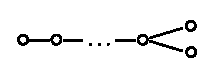
\includegraphics{344c.eps}}\\
$E_n, n = 6, 7, 8$ & {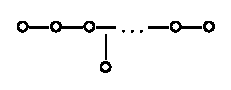
\includegraphics{344d.eps}}\\
$F_4$ & {
\includegraphics{344e.eps}}\\
$G^{(m)}_2$, $m \geqslant 5$ & {
\includegraphics{344f.eps}}\\
$H_3$ & {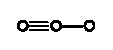
\includegraphics{344g.eps}}\\
$H_4$ & {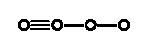
\includegraphics{344h.eps}}
\end{longtable}
\end{table}\pageoriginale

\begin{center}
%\fontsize{9}{11}\selectfont
\renewcommand{\arraystretch}{1.1}
\tabcolsep=10pt
%\setcounter{table}{0}
\begin{longtable}{@{}l@{\qquad\quad}l@{}}
\caption{Connected parabolic diagrams. (Lower index is equal to the rank)}\label{art10-table-2}\\
$\tilde{A_1}$ & {
\includegraphics{345a1.eps}}\\
$\tilde{A_n}, \; n \geqslant 2$ & {
\includegraphics{345a2.eps}}\\
$\tilde{B_n}, \; n \geqslant 3$ & {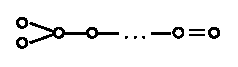
\includegraphics{345a3.eps}}\\
$\tilde{C_n}, \; n \geqslant 2$ & {
\includegraphics{345a4.eps}}\\
$\tilde{D_n}, \; n \geqslant 4$ & {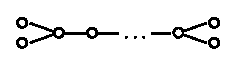
\includegraphics{345a5.eps}}\\
$\tilde{E}_6$ & {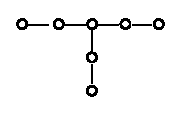
\includegraphics{345a6.eps}}\\
$\tilde{E}_7$ & {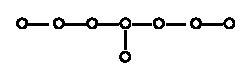
\includegraphics{345a7.eps}}\\
$\tilde{E}_8$ & {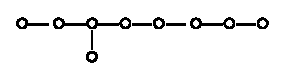
\includegraphics{345a8.eps}}\\
$\tilde{F}_4$ & {
\includegraphics{345a9.eps}}\\
$\tilde{G}_2$ & {
\includegraphics{345a10.eps}}\\
\end{longtable}
\end{center}


\pageoriginale
{
%\fontsize{9}{11}\selectfont
\renewcommand{\arraystretch}{1.5}
\tabcolsep=10pt
%\setcounter{table}{0}
\begin{longtable}{@{}l@{}}
\caption{Lanner's diagrams. ($n$ denotes the rank)}\label{art10-table-3}\\
 {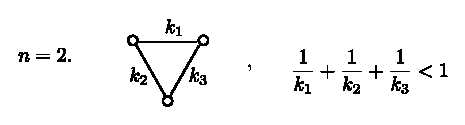
\includegraphics{345b.eps}}\\
 {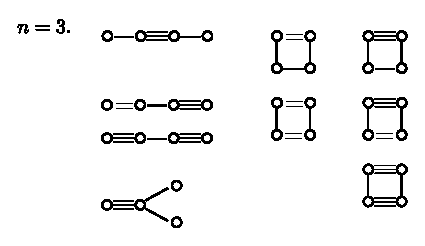
\includegraphics{345c.eps}}\\
{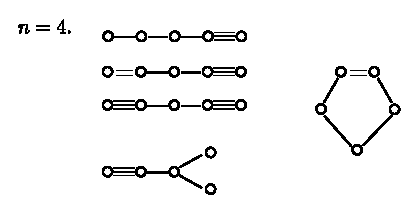
\includegraphics{345d.eps}}
\end{longtable}}\relax

\pageoriginale


\pageoriginale
\begin{landscape}
{
%\fontsize{9}{11}\selectfont
\renewcommand{\arraystretch}{1.2}
\tabcolsep=10pt
%\setcounter{table}{0}
\begin{longtable}{@{}ll@{}}
\caption{The diagrams of the maximal reflection subgroups of the groups of units of unimodular integral quadratic forms of signature $(n,1)$, $n \leqslant 17$. (The enumeration of vertices corresponds to the one in the text.)}\label{art10-table-4}\\
A. Odd Forms. & \\
 {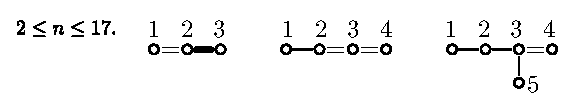
\includegraphics[scale=0.85]{344i.eps}} & \multirow{3}{4cm}{\raisebox{-1cm}{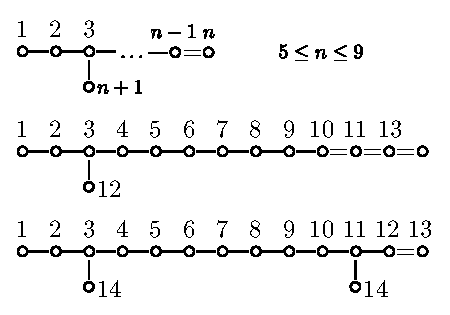
\includegraphics[scale=0.85]{345e.eps}}} \\ 
 {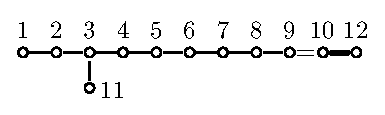
\includegraphics[scale=0.85]{344j.eps}} & \\
 {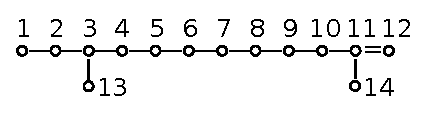
\includegraphics[scale=0.85]{344k.eps}} &\\
{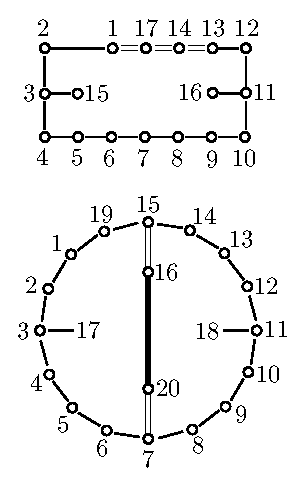
\includegraphics[scale=0.85]{346.eps}} & {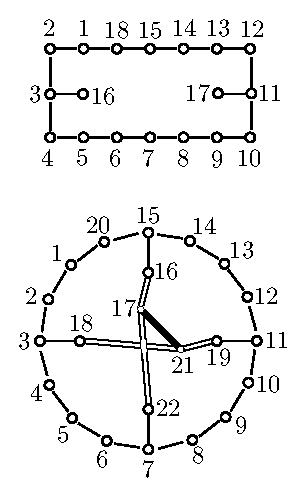
\includegraphics[scale=0.85]{347a.eps}}\\
B. Even Forms. $n = 9 , 17$.& \\
{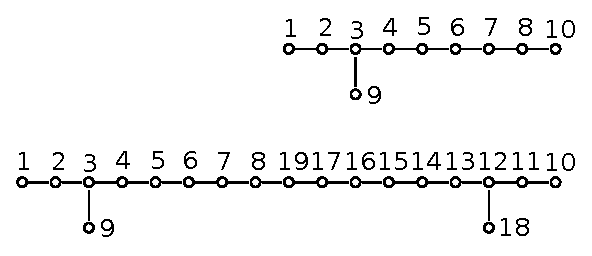
\includegraphics[scale=0.85]{347b.eps}} & \\
\end{longtable}}
\end{landscape}\relax

\begin{thebibliography}{99}
\bibitem{art10-key1} \textsc{H. S. M. Coxeter :} Discrete\pageoriginale groups generated by reflections, \textit{Ann. Math.,} 35, (1934), 588-621.

\bibitem{art10-key2} \textsc{C. L. Siegel :} Einheiten quadratischer Formen, \textit{Abh. Math. Sem. Univ. Hamburg,} 13 (1940), 209-239.

\bibitem{art10-key3} \textsc{F. Lanner :} On complexes with transitive groups of automorphisms, \textit{Lunds Univ. Math. Sem.,} 11 (1950).

\bibitem{art10-key4} \textsc{M. Kneser :} Klassenzahlen definiter quadratischer Formen, \textit{Arch. Math.,} 8, (1957), 241-250.

\bibitem{art10-key5} \textsc{J. H. Conway :} A characterization of Leech's lattice, \textit{Invent. Math., } 7, (1969), 137-142.

\bibitem{art10-key6} \textsc{J. -P. Serre :} \textit{Cours d'arithmetique}, Presses Universitaires de France, Paris, (1970).

\bibitem{art10-key7} \textsc{E. M. Andreev :} On convex polyhedra in Loba$\hat{\text{c}}$evski$\hat{\text{i}}$ spaces, \textit{Mat. Sbornik,} 81, (1970), 445-478.

\bibitem{art10-key8} \textsc{E. M. Andreev :} On convex polyhedra of finite volume in Loba$\hat{\text{c}}$evski$\hat{\text{i}}$ spaces, \textit{Mat. Sbornik,} 83, (1970), 256-260.

\bibitem{art10-key9} \textsc{E. M. Andreev :} On the intersection of the planes of faces of polyhedra with acute angles, \textit{Mat. Zametki,} 8, (1970), 521-527.

\bibitem{art10-key10} \textsc{\'E. B. Vinberg :} Discrete groups generated by reflections in Loba$\hat{\text{c}}$evski$\hat{\text{i}}$ spaces, \textit{Mat. Sbornik,} 78, (1967), 471-488.

\bibitem{art10-key11} \textsc{\'E. B. Vinberg :} Some examples of crystallographic groups in Loba$\hat{\text{c}}$evski$\hat{\text{i}}$ spaces, \textit{Mat. Sbornik,} 78, (1969), 633-639.

\bibitem{art10-key12} \textsc{\'E. B. Vinberg :} Discrete linear groups generated by reflections, \textit{Izv. Akad. Nauk SSSR, ser, mat., } 35, (1971), 1072-1112.

\bibitem{art10-key13} \textsc{\'E. B. Vinberg :} On the groups of units of some quadratic forms, \textit{Mat. Sbornik,}  87 (1972), 18-36.

\bibitem{art10-key14} \textsc{\'E. B. Vinberg :} On unimodular integral quadratic forms, \textit{Funkc. Analiz, } 6 (1972), 25-32.
\end{thebibliography}
